\documentclass{beamer}
\mode<presentation>
\usepackage{amsmath,amssymb,mathtools}
\usepackage{listings}
\usepackage{graphicx}
\usetheme{Boadilla}
\usecolortheme{lily}
\setbeamertemplate{footline}{
  \leavevmode%
  \hbox{%
  \begin{beamercolorbox}[wd=\paperwidth,ht=2ex,dp=1ex,right]{author in head/foot}%
    \insertframenumber{} / \inserttotalframenumber\hspace*{2ex}
  \end{beamercolorbox}}%
  \vskip0pt%
}
\setbeamertemplate{navigation symbols}{}
\lstset{
  frame=single,
  breaklines=true,
  columns=fullflexible,
  basicstyle=\ttfamily\tiny
}
\providecommand{\abs}[1]{\left\vert#1\right\vert}
\let\vec\mathbf
\title{Analog -- Problem 1.1.88}
\author{ee25btech11056 -- Suraj.N}
\begin{document}

\begin{frame}
  \titlepage
\end{frame}

\begin{frame}{Problem Statement}
The signal $x(t)$ is described by
\[
  x(t) = \begin{cases} 1 & -1 \leq t \leq +1 \\ 0 & \text{otherwise} \end{cases}
\]
Two of the angular frequencies at which its Fourier transform becomes
zero are: \hfill (EC 2008)

\begin{enumerate}
\item a) $\pi,\ 2\pi$
\item b) $0.5\pi,\ 1.5\pi$
\item c) $0,\ \pi$
\item d) $2\pi,\ 2.5\pi$
\end{enumerate}
\end{frame}

\begin{frame}{Key Concept: Fourier Transform}
The Fourier Transform of a continuous-time signal $x(t)$ is defined as:
\[
  X(j\omega) = \int_{-\infty}^{\infty} x(t)\, e^{-j\omega t}\, dt
\]
Since $x(t) = 1$ only on $[-1,+1]$ and zero elsewhere, the infinite
limits reduce to finite limits:
\[
  X(j\omega) = \int_{-1}^{+1} 1 \cdot e^{-j\omega t}\, dt
  = \int_{-1}^{+1} e^{-j\omega t}\, dt
\]
This is a standard rectangular pulse (rect function) of duration 2,
centred at $t = 0$. Its Fourier transform is a well-known sinc-type
result which we now derive explicitly.
\end{frame}

\begin{frame}{Evaluating the Integral}
For $\omega \neq 0$, integrate directly:
\[
  X(j\omega)
  = \left[\frac{e^{-j\omega t}}{-j\omega}\right]_{-1}^{+1}
  = \frac{e^{-j\omega} - e^{+j\omega}}{-j\omega}
  = \frac{e^{+j\omega} - e^{-j\omega}}{j\omega}
\]
Apply Euler's identity $\sin\theta = \dfrac{e^{j\theta}-e^{-j\theta}}{2j}$:
\[
  e^{+j\omega} - e^{-j\omega} = 2j\sin(\omega)
\]
Substituting:
\[
  \boxed{X(j\omega) = \frac{2\sin(\omega)}{\omega}}
\]
For $\omega = 0$:  integration,
$X(j0) = \displaystyle\int_{-1}^{1} dt = 2$.
\end{frame}

\begin{frame}{Finding the Zeros}
$X(j\omega) = \dfrac{2\sin(\omega)}{\omega} = 0$ requires:
\[
  \sin(\omega) = 0 \quad \text{and} \quad \omega \neq 0
\]
$\sin(\omega) = 0$ when $\omega = n\pi$ for integer $n \neq 0$.

So the zeros occur at:
\[
  \omega = \pm\pi,\ \pm 2\pi,\ \pm 3\pi,\ \ldots
\]

Now check each option against this zero set:
\begin{enumerate}
\item a) $\omega = \pi$ and $\omega = 2\pi$: both are integer multiples of $\pi$ \checkmark
\item b) $\omega = 0.5\pi$ and $\omega = 1.5\pi$: neither is an integer multiple of $\pi$
\item c) $\omega = 0$: $X(j0) = 2 \neq 0$, so 0 is not a zero
\item d) $\omega = 2.5\pi$: not an integer multiple of $\pi$
\end{enumerate}
\end{frame}


\begin{frame}{Conclusion}
The Fourier transform of the rectangular pulse $x(t)$ is:
\[
  X(j\omega) = \frac{2\sin(\omega)}{\omega}
\]
This function is zero whenever $\omega$ is a non-zero integer multiple
of $\pi$:
\[
  \omega = \pm\pi,\ \pm 2\pi,\ \pm 3\pi,\ \ldots
\]
Both $\omega = \pi$ and $\omega = 2\pi$ are zeros of $X(j\omega)$.

The correct answer is \textbf{a) $\pi,\ 2\pi$}.
\end{frame} 

\begin{frame}{Fourier Transform Plot} 

\begin{figure}[h!]
  \centering
  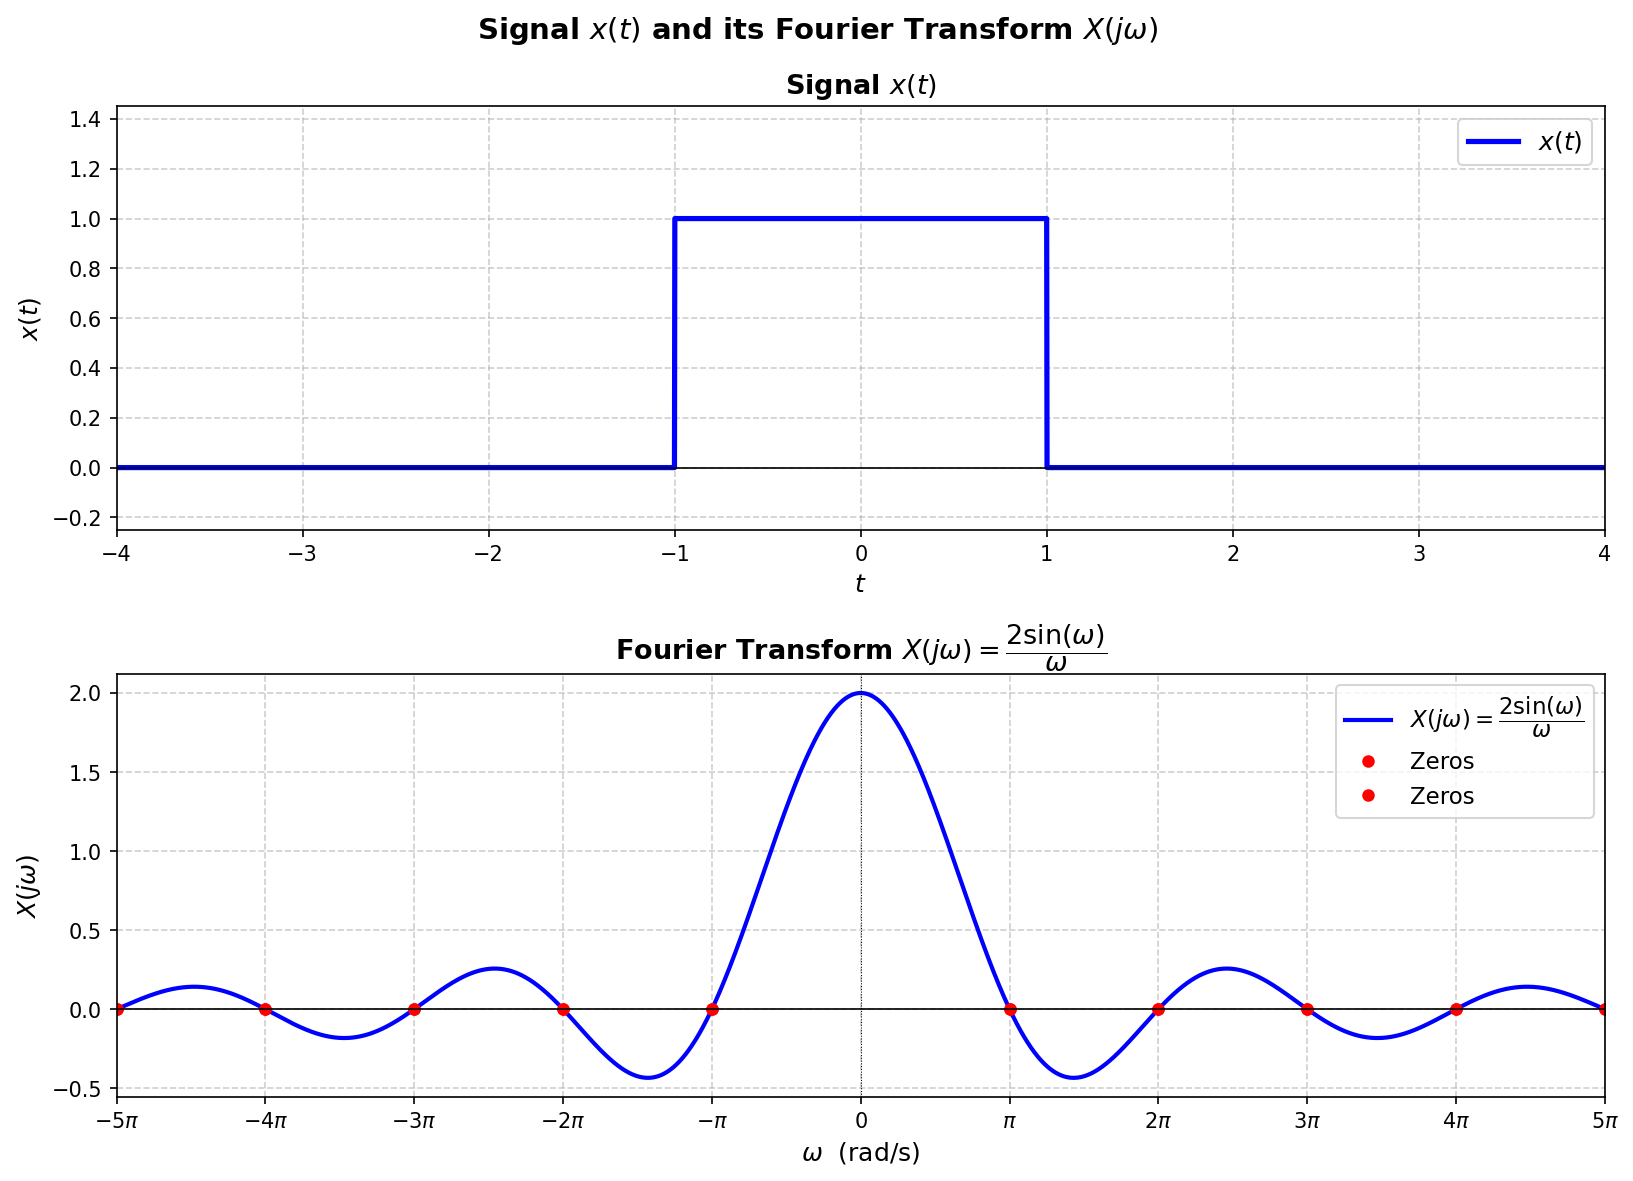
\includegraphics[width=0.8\columnwidth]{figs/fourier_transform_plot.png} 
  \caption{ Fourier Transform}
  \label{Fig1}
\end{figure}


\end{frame} 

\begin{frame}{Fourier Series Plot} 

\begin{figure}[h!]
  \centering
  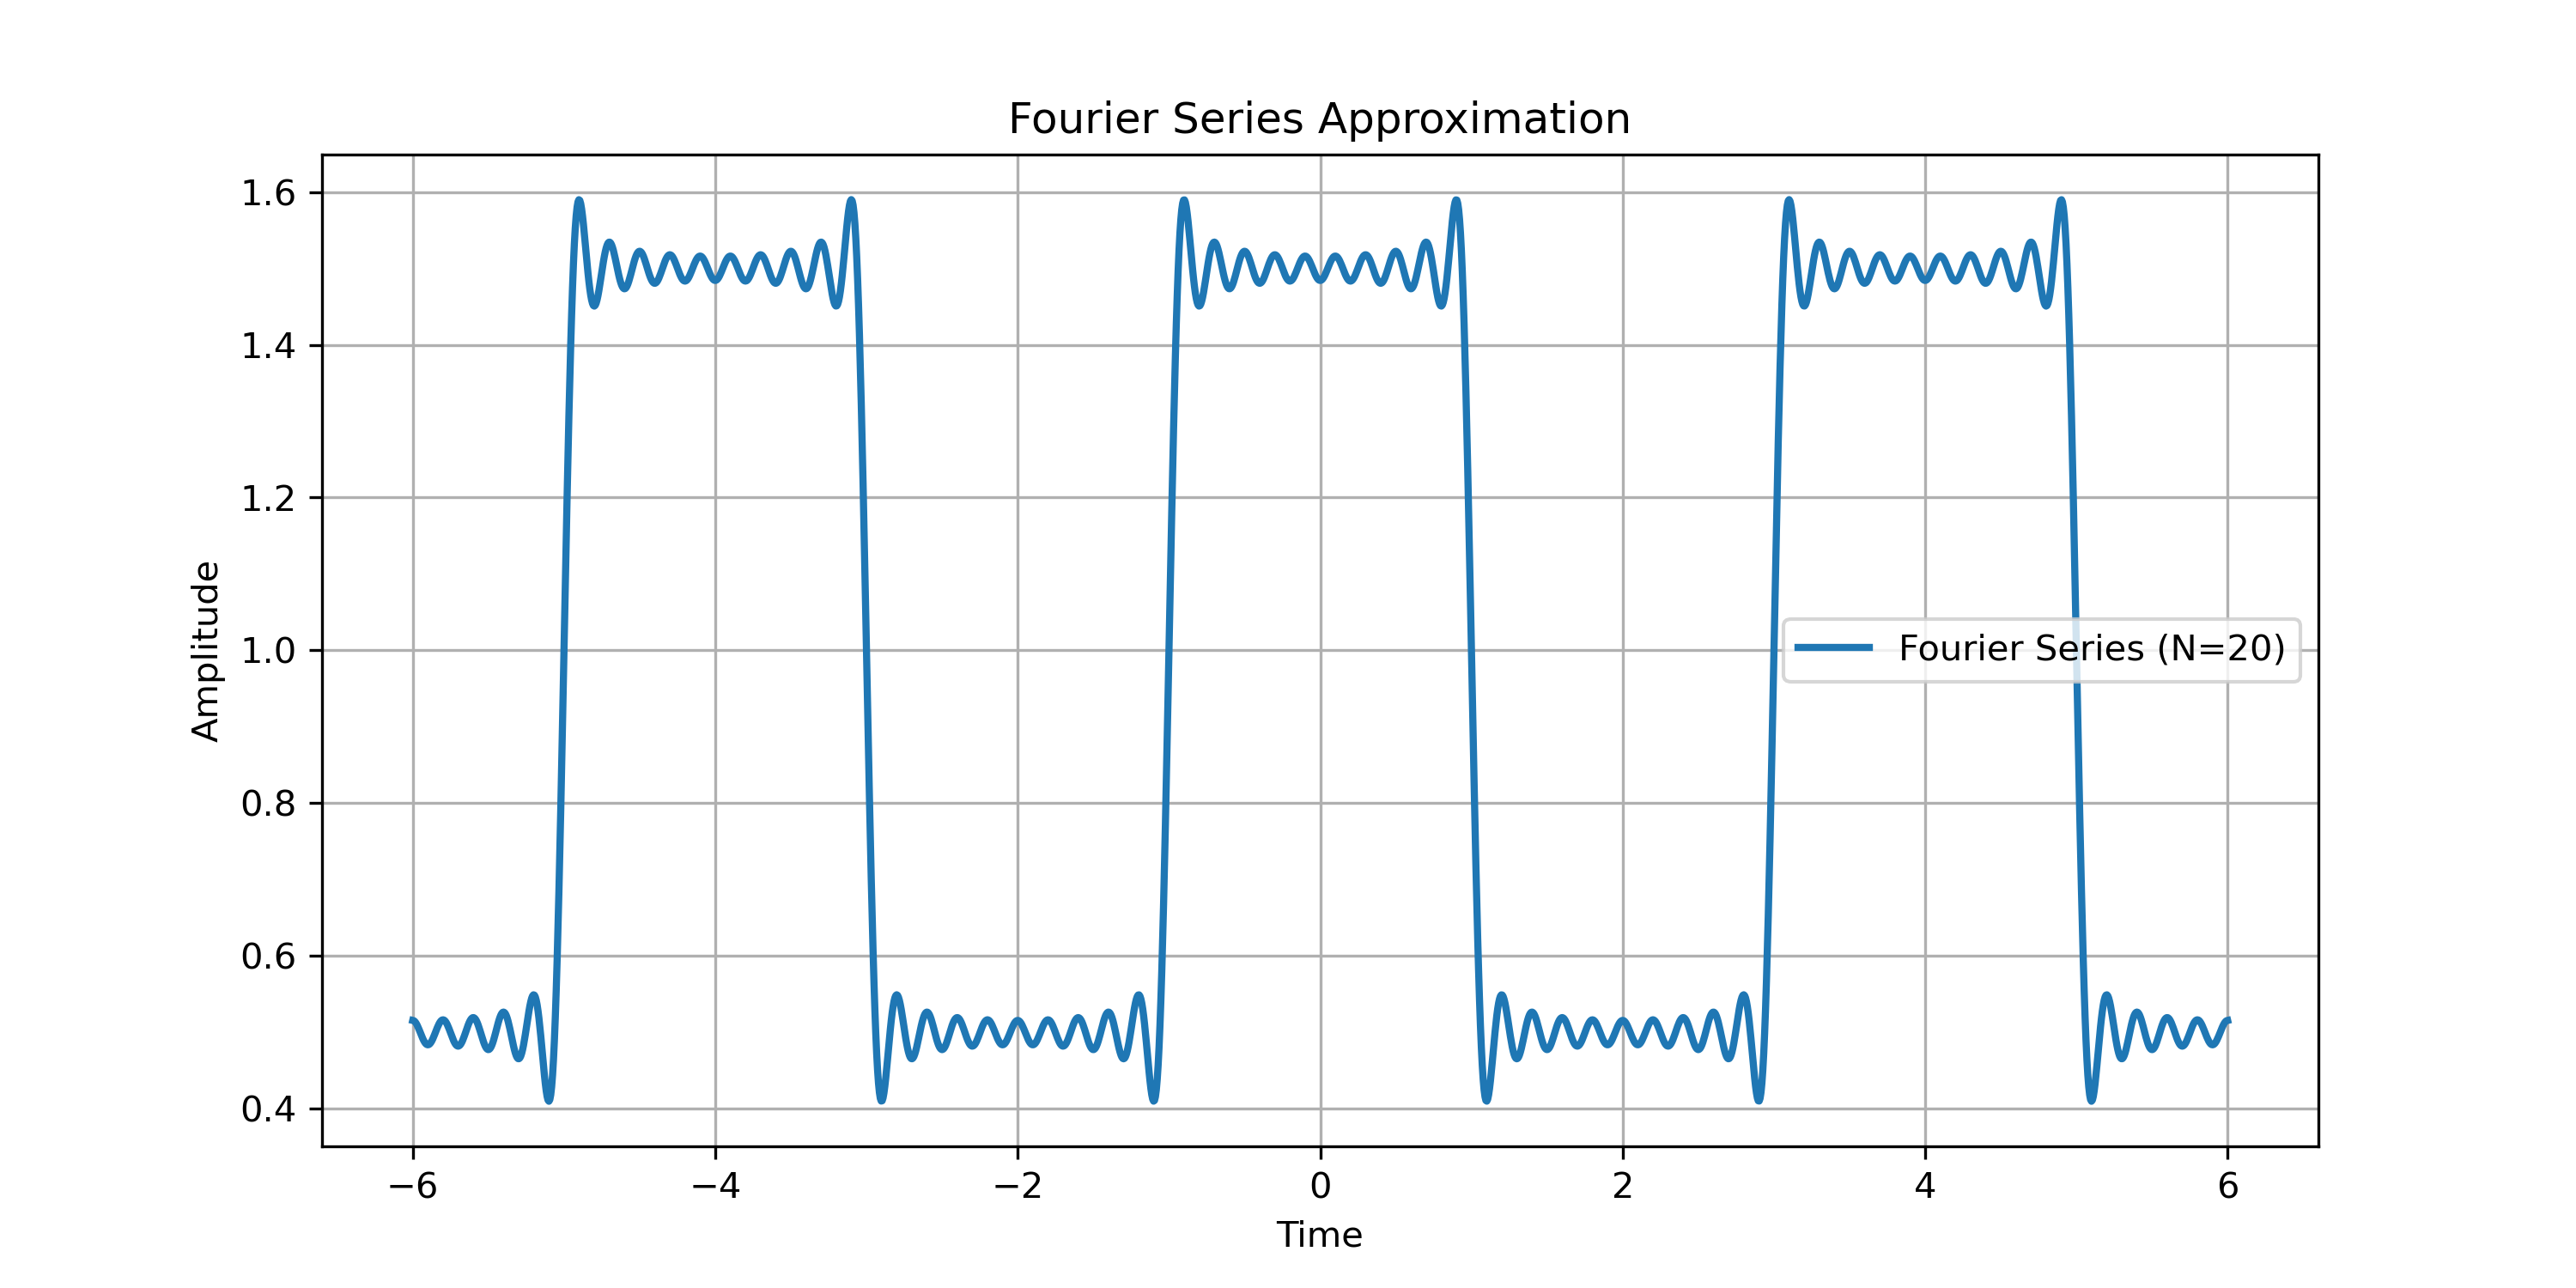
\includegraphics[width=0.9\columnwidth]{figs/fourier_series.png} 
  \caption{ Fourier Series}
  \label{Fig1}
\end{figure}


\end{frame} 



\begin{frame}[fragile]{Python Code: Verification}

\lstset{
    language=Python,
    basicstyle=\ttfamily\small,
    keywordstyle=\color{blue},
    commentstyle=\color{green!50!black},
    stringstyle=\color{red},
    numbers=left,
    numberstyle=\tiny,
    stepnumber=1,
    numbersep=8pt,
    showstringspaces=false,
    breaklines=true,
    breakatwhitespace=true,
    tabsize=4,
    frame=single,
    rulecolor=\color{black}
}

\begin{lstlisting}
import numpy as np
from scipy.integrate import quad
from sympy import symbols, integrate, exp, I, sin, pi, oo, And, Piecewise
from sympy import simplify, lambdify, re

print("=" * 55)
print("sympy -- symbolic Fourier Transform")
print("=" * 55)

t_s, w_s = symbols('t omega', real=True)

# Define x(t) 
x_sym = Piecewise((1, And(t_s >= -1, t_s <= 1)), (0, True))

# Compute FT 
Xw_sym = integrate(x_sym * exp(-I * w_s * t_s), (t_s, -oo, oo))
Xw_sym = simplify(Xw_sym)
print(f"\n  X(j*omega) = {Xw_sym}")
\end{lstlisting}
\end{frame}

\begin{frame}[fragile]{Python Code: Verification}

\lstset{
    language=Python,
    basicstyle=\ttfamily\small,
    keywordstyle=\color{blue},
    commentstyle=\color{green!50!black},
    stringstyle=\color{red},
    numbers=left,
    numberstyle=\tiny,
    stepnumber=1,
    numbersep=8pt,
    showstringspaces=false,
    breaklines=true,
    breakatwhitespace=true,
    tabsize=4,
    frame=single,
    rulecolor=\color{black}
}

\begin{lstlisting}


print("\n  Evaluating at option frequencies:")
for label, val in [("w = pi",    pi),
                   ("w = 2*pi",  2*pi),
                   ("w = 0.5pi", pi/2),
                   ("w = 1.5pi", 3*pi/2),
                   ("w = 0",     0)]:
    result = Xw_sym.subs(w_s, val)
    print(f"    {label:12s} -> X = {simplify(result)}")

print("\n" + "=" * 55)
print("scipy.integrate.quad -- numerical integration")
print("=" * 55)

\end{lstlisting}
\end{frame}

\begin{frame}[fragile]{Python Code: Verification}

\lstset{
    language=Python,
    basicstyle=\ttfamily\small,
    keywordstyle=\color{blue},
    commentstyle=\color{green!50!black},
    stringstyle=\color{red},
    numbers=left,
    numberstyle=\tiny,
    stepnumber=1,
    numbersep=8pt,
    showstringspaces=false,
    breaklines=true,
    breakatwhitespace=true,
    tabsize=4,
    frame=single,
    rulecolor=\color{black}
}

\begin{lstlisting}
def X_quad(w):
    """Compute X(jw) via direct numerical integration of x(t)e^{-jwt}"""
    if abs(w) < 1e-10:
        val, _ = quad(lambda t: 1.0, -1, 1)
        return val
    real_part, _ = quad(lambda t: np.cos(w * t), -1, 1)
    imag_part, _ = quad(lambda t: -np.sin(w * t), -1, 1)
    return complex(real_part, imag_part)

print("\n  Checking all four options:")
options = {
    "a) pi, 2pi"       : [np.pi,       2*np.pi],
    "b) 0.5pi, 1.5pi"  : [0.5*np.pi,   1.5*np.pi],
    "c) 0, pi"         : [0,            np.pi],
    "d) 2pi, 2.5pi"    : [2*np.pi,      2.5*np.pi],
} 

\end{lstlisting}
\end{frame}

\begin{frame}[fragile]{Python Code: Verification}

\lstset{
    language=Python,
    basicstyle=\ttfamily\small,
    keywordstyle=\color{blue},
    commentstyle=\color{green!50!black},
    stringstyle=\color{red},
    numbers=left,
    numberstyle=\tiny,
    stepnumber=1,
    numbersep=8pt,
    showstringspaces=false,
    breaklines=true,
    breakatwhitespace=true,
    tabsize=4,
    frame=single,
    rulecolor=\color{black}
}

\begin{lstlisting}
for opt, freqs in options.items():
    vals = [abs(X_quad(w)) for w in freqs]
    is_zero = all(v < 1e-9 for v in vals)
    print(f"  {opt}: |X|={vals[0]:.6f}, {vals[1]:.6f}  -> zeros={is_zero}")

print("\n  Answer: option a) is the only pair where both |X(jw)| = 0")
\end{lstlisting}
\end{frame}

\begin{frame}[fragile]{Python Code: Plotting}

\lstset{
    language=Python,
    basicstyle=\ttfamily\small,
    keywordstyle=\color{blue},
    commentstyle=\color{green!50!black},
    stringstyle=\color{red},
    numbers=left,
    numberstyle=\tiny,
    stepnumber=1,
    numbersep=8pt,
    showstringspaces=false,
    breaklines=true,
    breakatwhitespace=true,
    tabsize=4,
    frame=single,
    rulecolor=\color{black}
}

\begin{lstlisting}
import numpy as np
import matplotlib.pyplot as plt

# ── Analytical FT only ───────────────────────────────────────────
def X_analytical(w):
    with np.errstate(divide='ignore', invalid='ignore'):
        return np.where(np.abs(w) < 1e-9, 2.0, 2*np.sin(w)/w)

w    = np.linspace(-5*np.pi, 5*np.pi, 8000)
Xw   = X_analytical(w)

# ── Figure ───────────────────────────────────────────────────────
fig, axes = plt.subplots(2, 1, figsize=(11, 8))
fig.suptitle(
    r'Signal $x(t)$ and its Fourier Transform $X(j\omega)$',
    fontsize=14, fontweight='bold')
\end{lstlisting}
\end{frame}

\begin{frame}[fragile]{Python Code: Plotting}

\lstset{
    language=Python,
    basicstyle=\ttfamily\small,
    keywordstyle=\color{blue},
    commentstyle=\color{green!50!black},
    stringstyle=\color{red},
    numbers=left,
    numberstyle=\tiny,
    stepnumber=1,
    numbersep=8pt,
    showstringspaces=false,
    breaklines=true,
    breakatwhitespace=true,
    tabsize=4,
    frame=single,
    rulecolor=\color{black}
}

\begin{lstlisting}
# Top: x(t) -- single rect pulse, no fill colour
t_disp  = np.linspace(-4, 4, 4000)
xt_disp = np.where(np.abs(t_disp) <= 1.0, 1.0, 0.0)

axes[0].plot(t_disp, xt_disp, 'b-', linewidth=2.5, label=r'$x(t)$')
axes[0].set_title('Signal $x(t)$', fontsize=13, fontweight='bold')
axes[0].set_xlabel('$t$', fontsize=12)
axes[0].set_ylabel('$x(t)$', fontsize=12)
axes[0].set_xlim(-4, 4)
axes[0].set_ylim(-0.25, 1.45)
axes[0].axhline(0, color='k', linewidth=0.8)
axes[0].set_xticks(range(-4, 5))
axes[0].legend(fontsize=12)
axes[0].grid(True, linestyle='--', alpha=0.6)
\end{lstlisting}
\end{frame}

\begin{frame}[fragile]{Python Code: Plotting}

\lstset{
    language=Python,
    basicstyle=\ttfamily\small,
    keywordstyle=\color{blue},
    commentstyle=\color{green!50!black},
    stringstyle=\color{red},
    numbers=left,
    numberstyle=\tiny,
    stepnumber=1,
    numbersep=8pt,
    showstringspaces=false,
    breaklines=true,
    breakatwhitespace=true,
    tabsize=4,
    frame=single,
    rulecolor=\color{black}
}

\begin{lstlisting}
# Bottom: X(jw) 
axes[1].plot(w, Xw, 'b-', linewidth=2.0,
             label=r'$X(j\omega) = \dfrac{2\sin(\omega)}{\omega}$')
axes[1].axhline(0, color='k', linewidth=0.8)
axes[1].axvline(0, color='k', linewidth=0.5, linestyle=':')

tick_vals   = [n*np.pi for n in range(-5, 6)]
tick_labels = [r'$-5\pi$', r'$-4\pi$', r'$-3\pi$', r'$-2\pi$',
               r'$-\pi$',  r'$0$',     r'$\pi$',   r'$2\pi$',
               r'$3\pi$',  r'$4\pi$',  r'$5\pi$']
axes[1].set_xticks(tick_vals)
axes[1].set_xticklabels(tick_labels, fontsize=10)
axes[1].set_xlim(-5*np.pi, 5*np.pi)
axes[1].set_title(
    r'Fourier Transform $X(j\omega) = \dfrac{2\sin(\omega)}{\omega}$',
    fontsize=13, fontweight='bold')
axes[1].set_xlabel(r'$\omega$  (rad/s)', fontsize=12)
axes[1].set_ylabel(r'$X(j\omega)$', fontsize=12)
axes[1].legend(fontsize=11, loc='upper right')
axes[1].grid(True, linestyle='--', alpha=0.6)

plt.tight_layout()
plt.savefig('fourier_transform_plot.png', dpi=150, bbox_inches='tight')
print("Saved fourier_transform_plot.png")
\end{lstlisting} 
\end{frame}

\begin{frame}[fragile]{Python Code: Fourier Series}

\lstset{
    language=Python,
    basicstyle=\ttfamily\small,
    keywordstyle=\color{blue},
    commentstyle=\color{green!50!black},
    stringstyle=\color{red},
    numbers=left,
    numberstyle=\tiny,
    stepnumber=1,
    numbersep=8pt,
    showstringspaces=false,
    breaklines=true,
    breakatwhitespace=true,
    tabsize=4,
    frame=single,
    rulecolor=\color{black}
}

\begin{lstlisting}
import numpy as np
import matplotlib.pyplot as plt

# Parameters
N = 20                 # number of harmonics
T = 4                  # period
w0 = 2 * np.pi / T     # fundamental frequency

# Time axis
t = np.linspace(-6, 6, 2000)

# Fourier series approximation
x_fs = np.ones_like(t) * (2 / T) * 2   # a0/2 = 0.5

# Add cosine terms
for n in range(1, N + 1):
    an = (2 / (n * np.pi)) * np.sin(n * np.pi / 2)
    x_fs += an * np.cos(n * w0 * t)

\end{lstlisting} 
\end{frame}

\begin{frame}[fragile]{Python Code: Fourier Series}

\lstset{
    language=Python,
    basicstyle=\ttfamily\small,
    keywordstyle=\color{blue},
    commentstyle=\color{green!50!black},
    stringstyle=\color{red},
    numbers=left,
    numberstyle=\tiny,
    stepnumber=1,
    numbersep=8pt,
    showstringspaces=false,
    breaklines=true,
    breakatwhitespace=true,
    tabsize=4,
    frame=single,
    rulecolor=\color{black}
}

\begin{lstlisting}
# Plot 
plt.figure(figsize=(10, 5))
plt.plot(t, x_fs, label=f'Fourier Series (N={N})', linewidth=2)

plt.title('Fourier Series Approximation')
plt.xlabel('Time')
plt.ylabel('Amplitude')
plt.legend()
plt.grid()

# Save figure
plt.savefig('fourier_series.png', dpi=300)

plt.show()
\end{lstlisting} 
\end{frame}


\end{document}
